\subsection{IPFS}

\subsubsection{Infraestructura de despliegue}

En IPFS, es posible desplegar una aplicación web subiendo un directorio con todos los archivos estáticos necesarios para el funcionamiento en un navegador, incluyendo el código necesario a nivel aplicación. Esto se puede realizar manualmente mediante cualquier cliente de IPFS, como Kubo\cite{kubo} o Helia\cite{helia}, y devuelve un \textit{content identifier} (CID) \cite{cid} que representa esa versión de la aplicación.

Cualquier usuario puede publicar su sitio web en la red de IPFS a través de un nodo local de manera gratuita y poco tiempo. IPFS provee un tutorial en su página de cómo realizarlo \cite{ipfs-static-website}. A continuación se detallará las implicaciones que tiene desplegar una aplicación web de esta manera, y que alternativas existen para publicar en IPFS.

Al subir un archivo —por ejemplo, código HTML— su contenido se inserta en una función de hash, y así se obtiene su CID. Desde ese momento, cualquier nodo que desee obtener el archivo puede encontrarlo utilizando dicho CID. Sin embargo, no se asegura la persistencia del archivo, y dejará de ser accesible luego de un tiempo. Esto se debe al \textit{garbage collector} \cite{garbage-collector} implementado por IPFS, que desecha datos para liberar almacenamiento de forma arbitraria. Por esta razón existe el concepto de \cite{pinning}: \textit{"pinear"} o fijar un archivo o directorio significa instruir al nodo IPFS para que trate dicha información como esencial y, por lo tanto, no lo descarte. 

No obstante, fijar un archivo o directorio no asegura su disponibilidad indefinida en el tiempo, ya a que esta depende de que el nodo que que fije el contenido esté activo, o de que otros nodos que hayan accedido al archivo y aún lo tengan en su caché. Para mejorar la disponibilidad de un archivo, lo ideal es que varios nodos fijen el contenido, de modo que otro nodo que desee obtener el contenido pueda hacerlo desde cualquiera de ellos.

Para lograr que el contenido persista en la red sin necesidad de que el nodo local esté activo, existen opciones para delegar el pinning del archivo o directorio. Existen servicios de pinning, el servicio ofrecido por Filecoin, y clústeres colaborativos, que actúan fijando los archivos en múltiples nodos, aumentando no solo su disponibilidad sino también su distribución, y por ende logrando un acceso más rápido al contenido.

\paragraph{Servicios de \textit{pinning}}

La manera más fácil de asegurarse que los datos estén disponibles y se persistan es usar un servicio de \textit{pinning} \cite{pinning-services}. Estos servicios cuentan con varios nodos que fijan archivos. De esta manera, ya no es necesario contar con un nodo local que los aloje. Algunos ejemplos de servicios de pinning incluyen Fleek \cite{fleek}, Filebase\cite{filebase} y Pinata \cite{pinata}.

Estos servicios no van de la mano con la filosofía de aplicaciones estrictamente comunitarias. Por un lado, los servicios de \textit{pinning} tienen un modelo gratis con funcionalidad limitada o capacidad de almacenamiento limitado. Por otro lado, se depende de estos servicios, lo que en esencia centraliza el proceso de despliegue de la aplicación o sitio web. Si por algún motivo el servicio dejara de fijar los archivos, estos pueden dejar de estar disponibles en la red IPFS, e incluso pueden perderse por completo. Esto rompe completamente con la naturaleza de aplicaciones descentralizadas y pasa a tener una centralización tercerizada similar a utilizar un \textit{cloud hosting}.

\paragraph{Filecoin}

Filecoin \cite{filecoin} es una Blockchain creada por IPFS que ofrece una red en la cuál un nodo puede proporcionar almacenamiento a cambio de un incentivo económico en forma de criptomoneda. Utilizando esta alternativa, un cliente puede ofrecer FIL, la criptomoneda de Filecoin a cambio de asegurar que el contenido está alojado en un nodo proveedor de almacenamiento. Este nodo proveedor debe proporcionar diariamente prueba de que el contenido indicado está disponible.

Es distinto de los servicios de pinning vistos, ya que los nodos que proveen almacenamiento dentro de Filecoin no pertenecen necesariamente a una misma organización, sino que se distribuyen a lo largo de su red. Sin embargo, requiere una inversión constante para mantener la persistencia del contenido, y por lo tanto no es ideal como solución de almacenamiento permanente para una aplicación comunitaria.

\paragraph{Clústeres colaborativos}

Un \textit{clúster} es un grupo de nodos de IPFS que actúan en conjunto para fijar un contenido. Funcionan sincronizando su \textit{pin set}, o sea, su lista de archivos y directorios fijados en un momento dado. Un clúster \textit{colaborativo} sigue esta premisa, pero permite que los usuarios puedan colaborar con su nodo local para el pinning de la aplicación sin tener la posibilidad de modificar los archivos, la cuál es delegada a nodos especiales que tienen la capacidad de orquestar el clúster en conjunto. Así, se logra que la misma comunidad mantenga en servicio el mecanismo de despliegue de la aplicación, lo cuál es acorde a la filosofía de aplicaciones comunitarias.

Actualmente, esta alternativa es poco explorada, por lo tanto no existe una forma fácil de creación, seguimiento y descubrimiento de estos clústeres. IPFS cuenta con una página con clústeres conocidos con los cuales se puede colaborar \cite{collaborative-clusters}, pero la cantidad es limitada.

Por otro lado, el principal problema es que los clústeres obligan a los nodos a fijar la totalidad de sus archivos, lo cuál puede significar un uso excesivo de almacenamiento necesario para colaborar. Hacer \textit{sharding} sobre el pin set, o sea, fijar parte del contenido de un clúster, es posible utilizando los parámetros de \texttt{replicator\_min} y \texttt{replicator\_max} al agregar un pin, que fijan un límite mínimo y máximo sobre la cantidad de nodos que tienen ese pin. Sin embargo, no es recomendado para clústeres colaborativos debido a la falta de \textit{proof of storage} \cite{cluster-sharding} \cite{collaborative-clusters-setup}. Esto se debe a que, debido a la manera en la que fue diseñada la arquitectura de IPFS, un nodo no confiable puede falsificar la lista de archivos que está fijando, por lo que hay una posibilidad de que una parte del contenido no esté en ninguno de los nodos, y por ende el contenido esté incompleto.

\paragraph{Acceso y mutabilidad}

Para buscar un contenido, un nodo de IPFS realiza una búsqueda a través de su CID, el cual es único. Debido a que es único, el CID cambiará si el contenido del sitio web o aplicación web cambia, ya que el contenido será distinto. Esto vuelve el proceso de despliegue altamente impráctico, ya que se necesitaría compartir un nuevo CID cada vez que se actualice una página.

Este problema puede ser resuelto con la ayuda de \textit{punteros mutables}. Estos punteros son un objeto de IPFS que apunta a un CID determinado, previamente elegido por el usuario. El CID al que apunta el puntero puede ser cambiado, por lo tanto permiten compartir la dirección del puntero una única vez y actualizar el CID al cuál apunta cada vez que se haga un cambio.

\subparagraph{IPNS}

InterPlanetary Name System (IPNS) \cite{ipns} es un sistema que permite crear  punteros mutables y obtener su dirección en forma de CIDs conocidos como \textit{names} o \textit{nombres de IPNS}. Estos nombres de IPNS pueden considerarse como enlaces que pueden actualizarse, conservando al mismo tiempo la verificabilidad del content addressing.

Un nombre de IPNS es un hash de una \cite{ipns-hash} clave pública. Está asociado a un \textit{IPNS record} \cite{ipns-record} que contiene la ruta a la que se vincula, entre otra información. El titular de la clave privada puede firmar y publicar nuevos registros en cualquier momento.

Es posible utilizar IPNS con uno de estos posibles enfoques:
\begin{itemize}
    \item \textbf{Consistencia:} garantizar que los usuarios siempre resuelvan el último registro de IPNS publicado, a riesgo de no poder resolverlo.
    \item \textbf{Disponibilidad:} resolver un registro de IPNS válido, a costa de potencialmente resolver un registro desactualizado -o sea, con un CID previo.
\end{itemize}

El registro IPNS se encuentra a través de la \textbf{Distributed Hash Table} (DHT) \cite{dht}. Todos los nodos de IPFS participan alojando el contenido de la DHT de forma colaborativa. Por lo tanto, la DHT actúa como un "directorio" descentralizado, donde la clave pública es un identificador. Esta tabla ayuda a localizar el registro IPNS que apunta al contenido deseado, entre otras funciones. Para entender mejor cómo IPNS funciona se puede consultar la documentación de IPFS.

IPNS es una buena forma de obtener mutabilidad dentro de IPFS. Una vez que se aloja un contenido en IPFS y se apunta a él mediante un \textit{nombre} de IPNS, el mayor problema pasa a ser la manera de acceder a IPNS en sí. El hecho de que los nombres sean hashes alfanuméricos, y no nombres legibles o memorables para humanos, representa una dificultad adicional a la hora de alojar un sitio web al cuál los usuarios puedan acceder fácilmente. A continuación se analizará dos alternativas para solucionar este problema.

\begin{figure}[h]
\centering
\fbox{\texttt{/ipns/k51qzi5uqu5dhkdbjdsauuyk5iyq82uzpjb0is3x6oy9dcmmr8dbcezv7v9fya}}
\caption{Ejemplo de la dirección de un nombre de IPNS}
\end{figure}

\subparagraph{DNSLink}

IPNS no es la única forma de crear punteros mutables en IPFS. DNSLink \cite{dnslink} utiliza registros \textit{DNS TXT} para asignar un nombre DNS a una dirección IPFS como un CID o un nombre de IPNS. Se puede usarlos para que siempre apunten a la última versión de un objeto en IPFS.

DNSLink actualmente es más rápido que IPNS, utiliza nombres legibles por humanos y también puede apuntar a nombres de IPNS. A pesar de ello, tiene un problema muy fundamental y es que se utiliza el protocolo \textbf{DNS}, el cual tiene claras deficiencias con la filosofía de aplicaciones comunitarias.

La más importante es que, aunque DNS tenga claras ventajas, como ser un sistema distribuido y escalable, es también un sistema algo centralizado. Las autoridades centrales como \textit{ICANN} gestionan las raíces del DNS. Esto hace que un registro DNS sea fácil de censurar, a nivel de registrador como también a nivel \textit{ISPs}.

\subparagraph{ENS}

\textbf{Ethereum Name Service (ENS)} \cite{ens}, es el protocolo de nombres descentralizado que se basa en blockchain \textit{Ethereum}. Funciona de manera similar a DNS, en el sentido de que los nombres ENS resuelven a nombres legibles para humanos. Como esto se computa en la blockchain de Ethereum, es seguro, descentralizado y transparente. Está diseñado específicamente para traducir identificadores como direcciones de billeteras de criptomonedas, hashes, metadata, entre otros, incluyendo direcciones de IPFS.

Es posible configurar un registro ENS para que se resuelva automáticamente la dirección IPNS, proporcionando nombres legibles para humanos que son más fáciles de compartir y acceder, y solucionando el principal problema de IPNS hasta este punto. Además, cuando se quiera actualizar el contenido, no será necesario modificar el registro ENS en sí, ya que siempre se va a apuntar al mismo nombre de IPNS.

Cabe aclarar que adquirir un dominio ENS tiene un costo, que depende de varios factores \cite{ens-price}:
\begin{itemize}
    \item El largo del nombre. Un nombre con menos caracteres tiende a tener un valor mayor.
    \item Cuán reciente expiró la licencia del dominio. Si un dominio expiró recientemente, se le aplica un precio \textit{premium} que decrece con el tiempo. Un dominio con mayor uso aumenta su precio.
    \item El valor del gas actual, que depende de la congestión de la blockchain.
\end{itemize}

\subparagraph{Acceso desde un navegador}

Por último, se necesita una manera de acceder a los archivos alojados en IPFS. En navegadores que soportan IPFS y ENS —como Opera \cite{opera-ipfs} y previamente Brave \cite{brave-ipfs}— se puede acceder directamente. En la mayoría de los navegadores, sin embargo, esta no es una opción. Para lograr un mayor alcance que incluya estos navegadores, se requiere el uso de un \textit{Ethereum gateway} que entienda un dominio ETH, y un \textit{IPFS gateway} para lograr obtener el contenido de IPFS \cite{ipfs-gateway}.

Un IPFS gateway es un nodo que recibe requests HTTP que contienen una dirección de IPFS, busca el contenido en la red de IPFS, y lo devuelve en una HTTP response. Esto es útil tanto para archivos como para directorios. Algunas gateways tienen la funcionalidad de mostrar una página web de manera correcta cuando un directorio tiene la estructura indicada. Esto nos es particularmente útil para poder mostrar una página moderna de la misma manera que se haría utilizando un servidor HTTP.

Una lista de gateways disponibles puede obtenerse utilizando el Public Gateway Checker \cite{public-gateway-checker} proporcionado por IPFS.

\begin{figure}[h!]
    \centering
    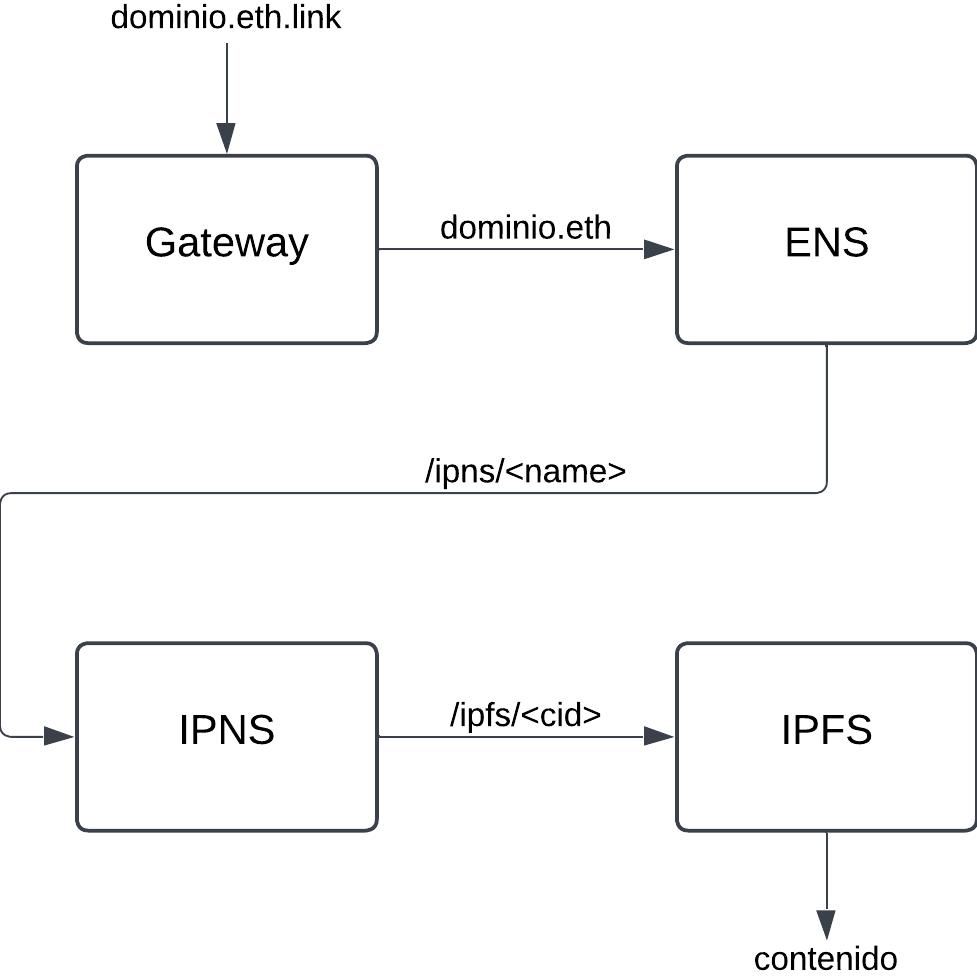
\includegraphics[width=0.5\linewidth]{img/solucion-ipfs/traduccion-dominio.png}
    \caption{Mapa de la traducción de un dominio al contenido de IPFS}
    \label{fig:traduccion-ipfs}
\end{figure}

En nuestro caso, se utilizó el servicio de Limo \cite{limo}, que soporta direcciones de ENS, y también recupera archivos de IPFS por lo que actúa como una gateway de ambos servicios. Para utilizarlo, simplemente se requiere agregar un sufijo \texttt{.link} al nombre de ENS. Por ejemplo, \texttt{dominio.eth} puede ser accedido mediante \texttt{dominio.eth.link}. A su vez, resuelve \texttt{dominio.eth} a una dirección de IPFS, y por lo tanto obtiene los archivos de esa dirección automáticamente.

\paragraph{Despliegue continuo}

En un proyecto de aplicación web centralizada, es común automatizar el proceso de despliegue con cada cambio que se realiza. Normalmente este proceso se activa con cada nuevo commit en una rama de Git especifica, e incluye todas las etapas necesarias para convertir el contenido de un repositorio Git en código estático listo para ser desplegado. También puede incluir más pasos que incluyan actualizaciones en el back-end.

Yendo al caso específico de aplicaciones web comunitarias, el script debe ser ejecutado en los nodos confiables, ya que una \textit{Github action} no puede utilizar un nodo IPFS que requiera puertos abiertos. En este tipo de aplicaciones, al tener una jerarquía mayormente horizontal, no hay un servidor central que orqueste esta actualización, sino que se necesita que cualquier nodo confiable pueda actualizar su contenido e instruir a los nodos colaborativos para actualizar su contenido de igual forma. Todo esto debe ser posible incluso cuando los nodos no reciben la actualización al mismo tiempo, es decir, no debe haber \textit{race conditions}.

Una forma de lograr esto es, por ejemplo, utilizar un algoritmo de elección de líder u otro algoritmo distribuido para elegir el nodo responsable de indicar al resto de los nodos el nuevo contenido a fijar. Sin embargo, esta manera de realizar la actualización implica una capa adicional de complejidad que no es necesaria debido a la naturaleza de IPFS.

Como ya se ha mencionado, si dos nodos suben el mismo contenido, obtendrán el mismo CID. Esto puede ser utilizado para que cualquier nodo confiable pueda actualizar el contenido y el nombre de IPNS independientemente del resto de los nodos confiables. Cuando se detecte un cambio nuevo, el nodo puede obtener el código estático, y acto posterior, indicar al resto de los nodos del clúster que fijen el CID especifico. En el caso de que sea el primer nodo en detectar el cambio, deberá instruir al resto del clúster para que dejen de fijar el CID antiguo. En el caso en que otro nodo haya detectado la actualización antes, no deberá actualizar ningún pin del clúster debido a que el mismo CID ya va a estar presente en la lista de pins.

\paragraph{Compilación}

Las herramientas de compilado no siempre son deterministas en los archivos compilados que genera. \texttt{Next.js}, por ejemplo, genera diferentes archivos estáticos en dos compilaciones basadas en el mismo código fuente. Esto es un problema para el enfoque propuesto, debido a que si dos nodos compilan el mismo código, el CID puede ser diferente. Para mitigar esto, se decidió hacer uso de un \textit{hook} que compile el código con cada \textit{commit} en la rama principal una única vez por cambio realizado. De esta manera, los nodos confiables pueden detectar el cambio en la rama utilizada para alojar los archivos estáticos, y hacer \textit{pull} sobre esos archivos y, por lo tanto, obtener un mismo CID.

\paragraph{Jerarquía}

En base a este análisis, podemos concluir que la mejor forma de desplegar una página web estática en IPFS es a través del uso de un clúster colaborativo compuesto por nodos que se integren con el proyecto de Git dado, así como una dirección IPNS a la cuál actualizar cada vez que hay un cambio, y un registro ENS para traducir la dirección IPNS a un nombre legible.

Como el nombre de IPNS cambiará a lo largo del tiempo en tanto se realicen cambio en el proyecto, se vuelve necesario seleccionar un grupo de nodos que se les confíe con tal fin. Esto se debe a que, de lo contrario, un posible atacante podría modificar el registro para invalidarlo o cambiar el contenido al que apunta. Por la misma razón, no cualquier nodo dentro del clúster debe ser capaz de cambiar el \textit{pin set}, o lista de CIDs fijados por el clúster.

IPFS Cluster tiene en cuenta esto, y hace la distinción entre un nodo \textit{trusted} y un nodo \textit{follower} para su implementación de clústeres \textit{colaborativos}\cite{ipfs-cluster-collaborative}. Para esta herramienta, se utiliza las denominaciones de nodo confiable y nodo colaborador, respectivamente.

\subparagraph{Nodo confiable} Este nodo tiene la capacidad de modificar el nombre IPNS, como también actualizar la configuración del mismo, y el \textit{pin set}. Son una parte esencial del clúster, ya que sin estos nodos no se podrá modificar el contenido. Esto no supone una desventaja ni tampoco hace que la solución se vuelva centralizada en el grupo de nodos confiables actual, debido a que los usuarios de la comunidad pueden crear su propio grupo de nodos confiables y actualizar el contenido por su cuenta, similar a realizar un \textit{fork} en un proyecto de Github.

\subparagraph{Nodo colaborador} Únicamente se encarga de fijar los archivos establecidos por los nodos confiables, y actualizar su \textit{pin set} cuando se lo indique. Al igual que los nodos confiables, debe fijar la totalidad de los archivos. Su finalidad es aumentar la disponibilidad del contenido y evitar que la información se pierda.

En un escenario ideal, existen varios nodos confiables disponibles en simultáneo. Esto previene un posible \textit{single point of failure} y asegura que el clúster siempre se encuentre en un estado válido.

\paragraph{Configuración} Para que un usuario pueda conectarse y contribuir como colaborador a un clúster, la herramienta de terminal \texttt{ipfs-cluster-follow} \cite{ipfs-cluster-follow} requiere una dirección de IPFS de la cuál obtener el archivo \texttt{service.json} \cite{service-json}. Este archivo de configuración contiene todos los datos necesarios para que un colaborador pueda unirse. Además, está sujeto a modificaciones, debido a que el archivo contiene las \textit{multiaddresses} \cite{multiaddr} de cada nodo confiable en forma de lista, por lo que agregar o remover un nodo confiable implica modificar el archivo. Es por esto que el proceso de despliegue también debe incluir este archivo. Desde la detección de una actualización en un repositorio de Git que lo contenga, el fijado del nuevo \texttt{service.json} al clúster, hasta la actualización de un nombre de IPNS que pueda distribuirse a los usuarios que quieran colaborar.

\begin{figure}[h]
\centering
\fbox{\texttt{/ip4/123.123.123.123/udp/9096/quic/p2p/12D3KooWLw...yPcuZJR}}
\caption{Ejemplo de una \textit{multiadress} posible que utiliza el protocolo QUIC.}
\end{figure}

\paragraph{Limitaciones}

Este enfoque, a cambio de ofrecer una solución comunitaria y descentralizada, tiene desventajas o aspectos a mejorar:

\subparagraph{Necesidad de tener nodos confiables} Estos nodos van a ser los encargados de administrar el clúster, y actualizar el IPNS. La distinción entre nodos confiables y nodos colaborativos es necesaria para evitar que un potencial atacante pueda modificar el CID al que apunta el nombre de IPNS, o modificar el contenido que fija el clúster colaborativo.
 
\subparagraph{Actualización del contenido} Por cada cambio que se realice en el directorio de la página, se deberá fijar el nuevo contenido al clúster, y por lo tanto todos los colaboradores tendrán que obtener todo el directorio nuevamente. Esto puede claramente volverse costoso con contenido de tamaño considerable.
    
\subparagraph{Cache de IPNS} El parámetro TTL de IPNS indica cuanto 'vive' un valor asociado a un nombre de IPNS en la cache de un nodo antes de forzar a este a volver a buscar el valor en la DHT. El problema que tiene esto es que, si se pone un valor muy elevado, un nodo gateway no buscará la actualización hasta que se cumpla el periodo y por lo tanto el registro de IPNS no se actualizará. Por otro lado, si se elige un valor muy corto, siempre se buscará el valor en la DHT, generando latencia al no utilizar el cache disponible. Pero a su vez, el nombre de IPNS en un nodo siempre tendrá la última versión que encuentre.

\subparagraph{Claves privadas compartidas} Cómo la actualización de un nombre de IPNS está firmada con una clave privada, todos los nodos confiables deberán tener la misma clave para poder potencialmente actualizar el registro IPNS y así evitar tener un único nodo con esa responsabilidad. Esto elimina un punto de falla único, pero aumenta las chances de que esa clave privada llegue a manos de un posible atacante.

\subparagraph{Apertura de puertos} IPFS Cluster utiliza el puerto 9096 para la comunicación entre nodos, el cual se tiene que abrir para un correcto funcionamiento. Esto puede suponer un esfuerzo adicional para usuarios que deseen colaborar.

\paragraph{Implementación}

Una vez explicado el análisis inicial y las decisiones que se tomaron para poder lograr un servicio que automatice y facilite parte del despliegue de una aplicación web, se detallará la solución realizada para el nodo confiable. El resultado es una herramienta que se puede levantar utilizando un comando, y automáticamente publique el contenido ubicado en el repositorio de Git dado, encargándose de mantenerlo disponible, de orquestar el \textit{pin set} del clúster, y detectar cambios. El repositorio se puede encontrar en el repositorio de GitHub \cite{repo-trusted-peer}.

\subparagraph{Arquitectura general}

La herramienta está compuesta por tres contenedores:
\begin{itemize}
    \item \textbf{Kubo:} el nodo de IPFS encargado de conectarse a la red de IPFS para publicar y obtener el contenido necesario.
    \item \textbf{IPFS Clusters:} gestiona el contenido fijado y coordina con otros nodos del clúster.
    \item \textbf{Watcher:} observa los repositorios de Git del proyecto y del archivo \texttt{service.json}, y orquesta acciones en los otros dos contenedores.
\end{itemize}

Todos los contenedores están orquestados mediante Docker Compose. El contenedor watcher está basado en Alpine Linux y utiliza scripts de shell portables. La comunicación entre contenedores se realiza mediante sus respectivas APIs HTTP \cite{kubo-api} \cite{cluster-api}.

\begin{figure}[h!]
    \centering
    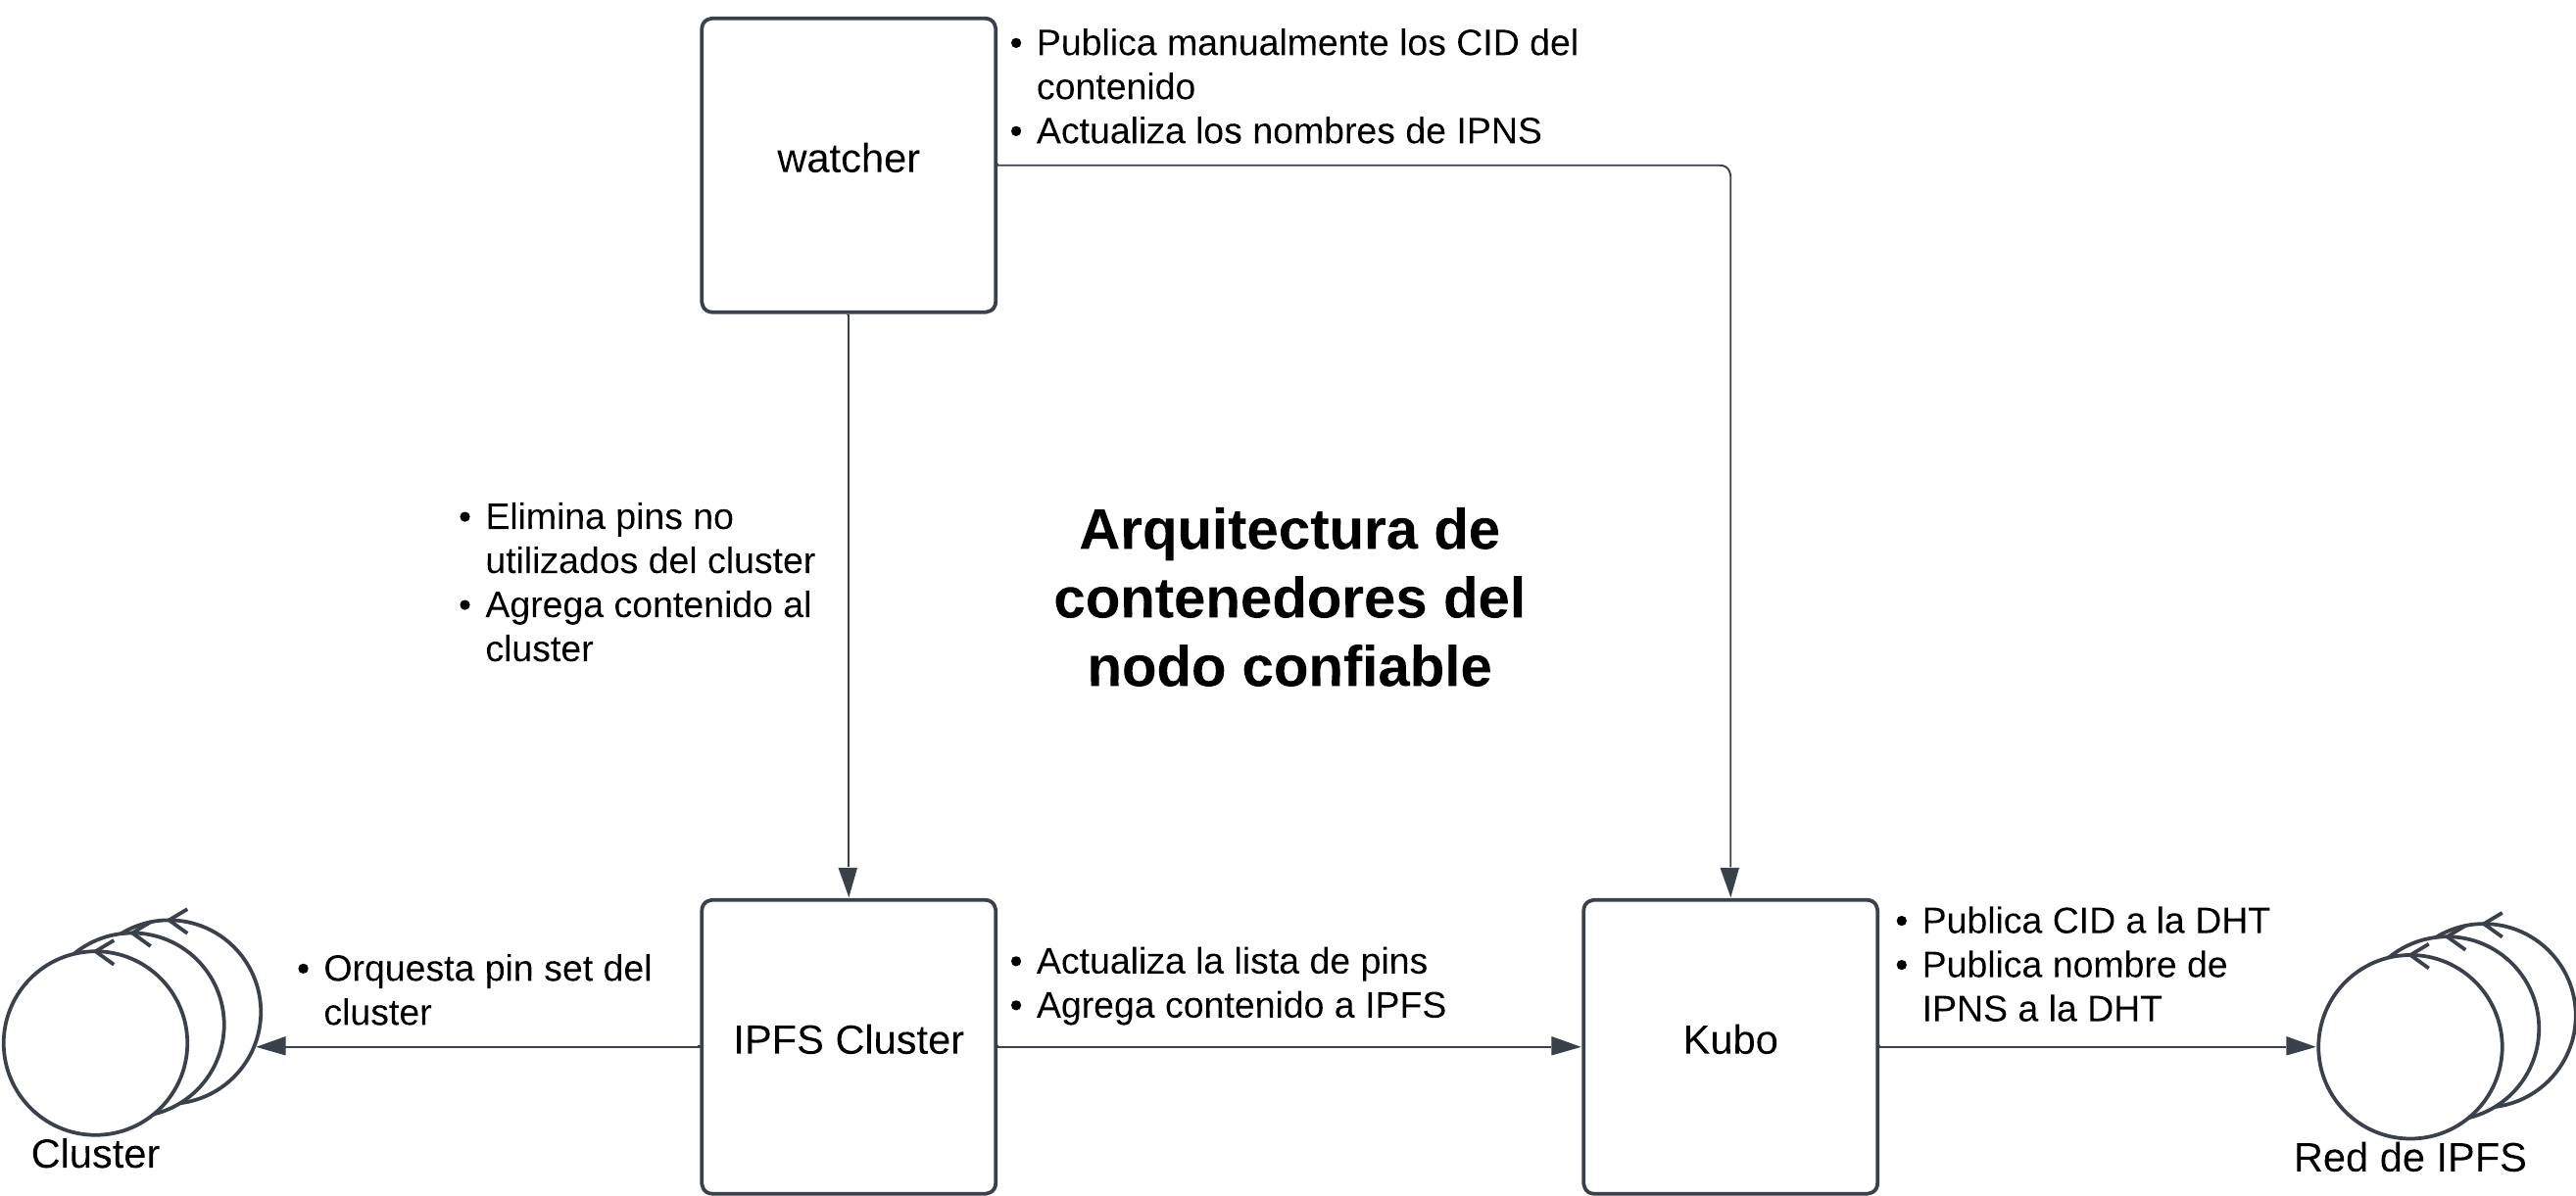
\includegraphics[width=1\linewidth]{img/solucion-ipfs/contenedores-trusted-peer.png}
    \caption{Mapa de interacciones entre los contenedores del nodo confiable}
    \label{fig:contenedores-trusted-peer}
\end{figure}

\subparagraph{Funcionamiento del Watcher} Este módulo del nodo confiable utiliza Git para comparar el último commit de la rama remota contra una copia local que se clona cada vez que se inicia. De esta manera, puede detectar cuando un nuevo cambio ocurre (tanto en el contenido como en \texttt{service.json}), e iniciar el proceso para obtener el nuevo cambio y desplegarlo. Dicho proceso se compone de los siguientes pasos:
\begin{enumerate}
    \item Subir el contenido y el \texttt{service.json} al Cluster, y obtener ambos CIDs.
    \item En base a los CIDs obtenidos, publicar ambos manualmente utilizando Kubo.
    \item Esperar a que todos los nodos dentro del clúster hayan fijado los nuevos CIDs.
    \item Actualizar los dos nombres de IPNS para que apunten a los nuevos CIDs.
    \item Eliminar los pins antiguos del clúster.
\end{enumerate}

\begin{figure}[h!]
    \centering
    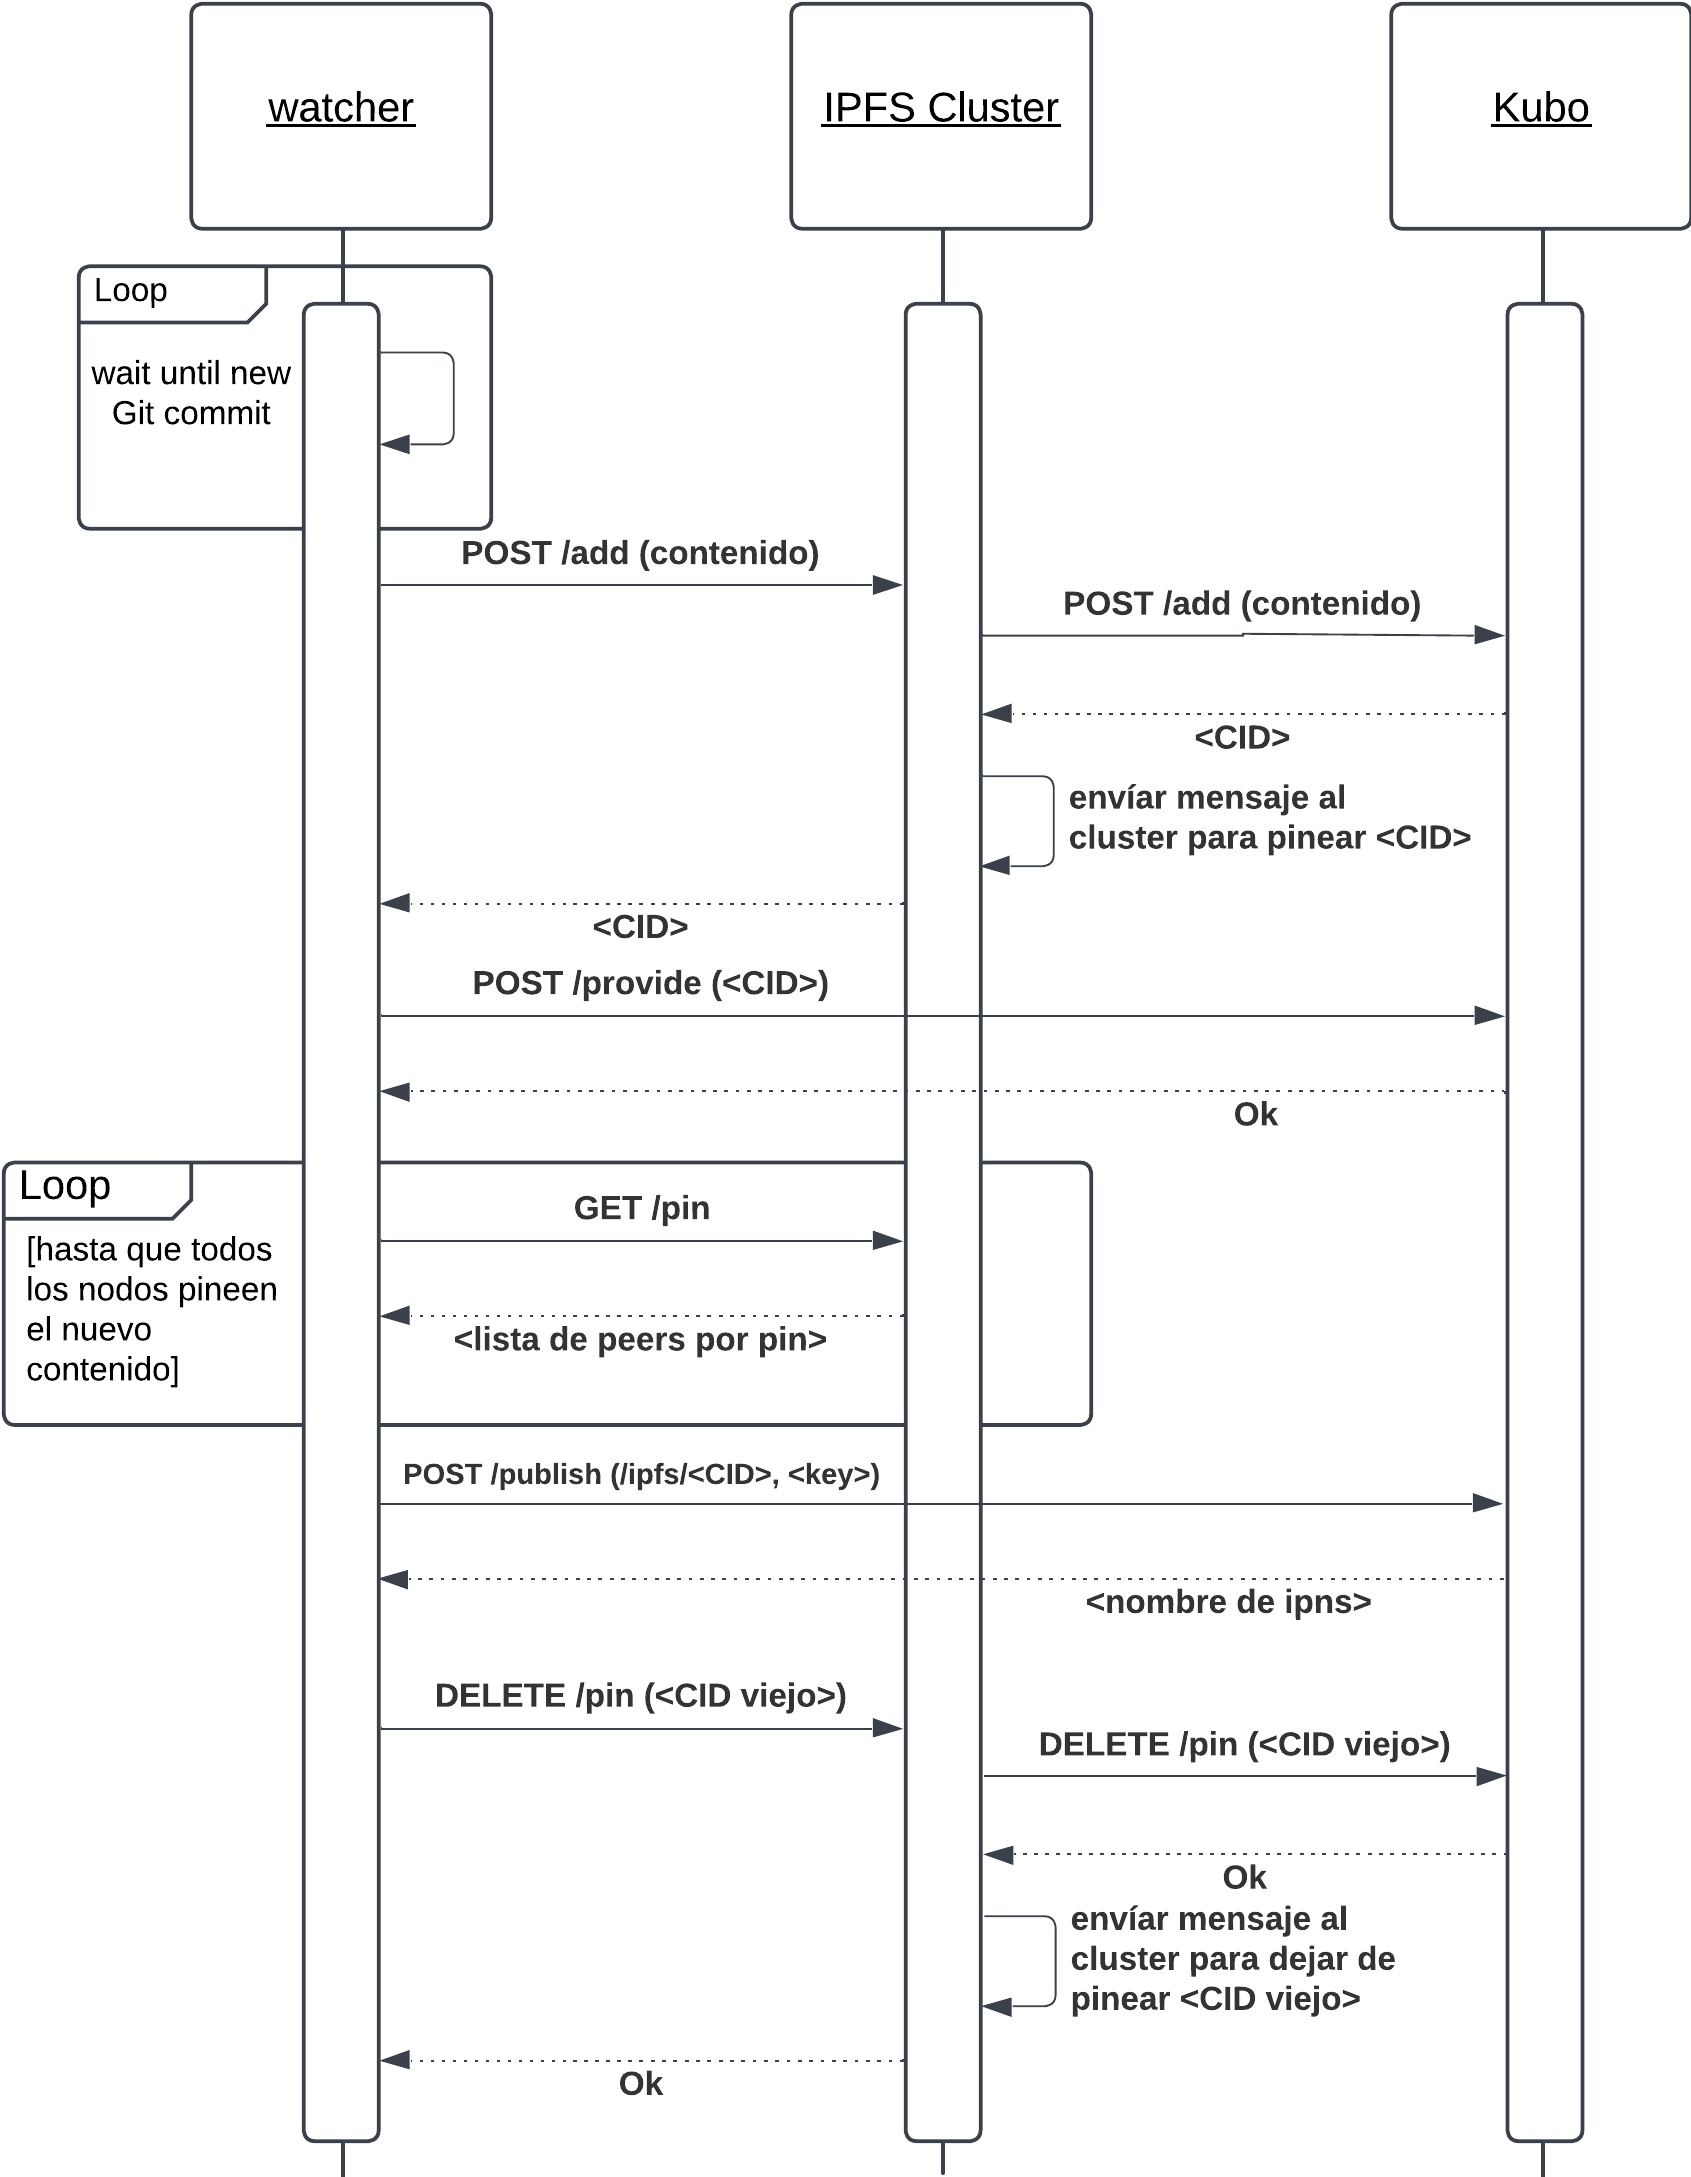
\includegraphics[width=0.5\linewidth]{img/solucion-ipfs/ds-trusted-peer.png}
    \caption{Diagrama de secuencia para el caso en que watcher detecta un cambio. Notar que para mayor claridad se omite los pasos para desplegar el nombre de IPNS del \texttt{service.json}, al ser exactamente los mismos que en el caso de un contenido.}
    \label{fig:contenedores-trusted-peer}
\end{figure}

\subparagraph{Disponibilidad} En el proceso mencionado para desplegar los cambios, existen dos factores que pueden afectar a la disponibilidad del contenido luego de recibir una actualización.

Por un lado, el nombre de IPNS puede no haberse actualizado en todos los nodos de la DHT, lo que provoca que algunos nodos apunten a la versión anterior del contenido. Esto se soluciona asegurándose de publicar el nuevo valor del nombre de IPNS \textbf{antes de instruir al clúster} para que deje de fijar la versión anterior.

Por otro lado, el contenido nuevo puede no estar disponible inmediatamente, ya que la publicación del CID en la DHT por parte del clúster se realiza de manera asíncrona. Para solucionar esto, se optó por publicar manualmente el CID con Kubo, de forma secuencial, antes de actualizar el nombre de IPNS. La desventaja de este enfoque es el tiempo adicional requerido para publicar el contenido, a cambio de garantizar su disponibilidad en todo momento, ya sea en su versión actual o en la nueva.

\subparagraph{Persistencia de la identidad del nodo}

Sabiendo que para ser un nodo confiable se debe tener su multiaddress en el archivo de \texttt{service.json}, es conveniente mantener el mismo PeerID a lo largo del tiempo y en distintas ejecuciones de la herramienta. Para ello, se debe indicar una \textit{identidad} que consiste de un PeerID, y una clave privada. Esto asegura que el nodo siempre se inicie con la misma identificación.

\subparagraph{Gestión de claves de IPNS}

Debido a la naturaleza de IPNS, un nombre solo puede ser modificado por un nodo que posea una clave privada determinada. Por ello, todos los nodos confiables deben tener las mismas clave privada de IPNS, una para el contenido y otra para \texttt{service.json}.

Para facilitar la inicialización, la herramienta provee un script que ayuda a generar la configuración y obtener los parámetros necesarios paso a paso. Esto incluye una identificación para el nodo, claves para IPNS, las direcciones de los repositorios de Git, y la IP pública necesaria para conectar los nodos a la red de IPFS.

\subparagraph{Integración con Git}

La manera en la que el contenedor \textit{watcher} puede detectar un cambio en el repositorio es consultando el repositorio remoto de Git cada minuto para identificar un cambio realizado y accionar el script de despliegue. Se requiere que el repositorio del contenido sea público, ya que la identificación por SSH o usuario y clave no están disponibles fácilmente dentro de un contenedor. De todas maneras, el contenido o archivos estáticos en el caso de una aplicación web ya son públicos por naturaleza, y debido al enfoque comunitario dado, que un repositorio necesite ser público no representa una restricción apreciable.

\subparagraph{Resultado}

La solución implementada logra automatizar el despliegue y la publicación de contenido en IPFS de forma confiable, simplificando muchos aspectos de IPFS y los clústeres colaborativos. Mediante un comando \texttt{make up} se levanta un nodo confiable que automáticamente puede desplegar y mantener actualizado el contenido que se desee. Cabe destacar que, si bien el enfoque está diseñado para aplicaciones web, esta herramienta permite el despliegue de cualquier tipo de contenido, como repositorios, documentación, etcétera.

Combinando esta herramienta junto con un dominio ENS y un gateway con el cuál acceder al contenido, se obtiene una aplicación web cuyo uso es equiparable a la de un servidor HTTP moderno, sin diferencias perceptibles para el usuario, y de manera comunitaria, descentralizada, y económica.

\subsubsection{Infraestructura de aplicación}

Para aplicaciones que requieran mantener un estado y permitir que usuarios puedan modificarlo, no es suficiente con la infraestructura que explicamos anteriormente, ya que no hay una noción de estado y solo se le permite cambiar su contenido a los dueños de lo que se despliega. Es por eso que es necesaria otra infraestructura, la cual nos provea de esas necesidades.

Esta infraestructura surgió en base a un extenso desarrollo del cual nos ayudó a entender y encontrar la abstracción de lo que se estaba creando. Al principio del desarrollo, esta era gran parte de la arquitectura del primer caso de uso no estático que realizamos, el repositorio de conocimiento, para luego convertirse en una implementación propia, la cual llamamos \textbf{AstraDB}.

A continuación pasaremos a explicar cómo es la arquitectura que compone a AstraDB, cómo fue su evolución y que decisiones se tomaron a lo largo de su desarrollo, como también cómo podemos hacer uso de ella para fácilmente crear las aplicación que venimos a analizar, aplicaciones comunitarias, distribuidas y descentralizadas dentro del ecosistema de IPFS, tal como lo son el repositorio de conocimiento y el mensajero en tiempo real, las cuales hacen uso de AstraDB para su funcionamiento.

\paragraph{Etapa de investigación}

Al comenzar con el desarrollo del repositorio de conocimiento nos encontramos con un desafío, cómo podemos lograr que una aplicación dentro del ecosistema de IPFS pueda tener, modificar y guardar un estado.

Dada la naturaleza de IPFS, como explicamos anteriormente, no está pensado para alojar cambios en tiempo real. El modelo de direccionamiento por contenido implica que cualquier modificación genera un nuevo identificador (CID), lo que resulta inconveniente para actualizar un recurso directamente sin mecanismos adicionales. Por esta razón, utilizar únicamente el conjunto de protocolos que IPFS ofrece no nos resulta conveniente para aplicaciones dinámicas.

Como sucede con un caso de uso muy similar al repositorio de conocimiento que queremos implementar, el proyecto de \textbf{Distributed Wikipedia Mirror}\cite{distributed-wikipedia-mirror}, el cual consistió en poner una versión de wikipedia en IPFS, únicamente funciona como versión Read-Only, y con snapshots manuales, lo cual es totalmente posible de hacer con la infraestructura que explicamos anteriormente.

Es por esto que resulta de un verdadero desafío lograr que una versión Read-Write sea posible sin sacrificar los principios de decentralización que IPFS nos provee. Para abordar esta limitación nos llevó a buscar herramientas complementarias dentro del ecosistema y ahí fue cuando nos encontramos con \textbf{OrbitDB}\cite{orbitdb}.

\paragraph{Representación de los datos}

OrbitDB es una base de datos peer-to-peer, distribuida y sin un servidor central. Utiliza IPFS para el almacenamiento de datos y \textbf{Libp2p}\cite{libp2p} para sincronizar automáticamente las bases de datos con otros peers. Es una base de datos \textbf{eventualmente consistente} que utiliza Merkle-CRDTs para escrituras y fusiones de base de datos libres de conflictos, lo que hace que OrbitDB sea una excelente opción para aplicaciones p2p y descentralizadas.
% , y en nuestro caso, para una wiki decentralizada.

OrbitDB ofrece varios tipos de bases de datos para diferentes modelos de datos y casos de uso. Algunos que se asemejan más a bases de datos convencionales, como puede ser un simple key-value y otros más distintos como puede ser uno de eventos secuenciales.

Uno de los requisitos de la infraestructura desarrollada es lograr una verdadera descentralización, significando que no haya una entidad o persona con mayores permisos sobre el resto, esto se traduce, en parte, a permitir que cualquiera que quiera pueda crear y/o modificar la base de datos sin ninguna restricción. Para lograr esto, OrbitDB nos permite indicar que cualquier nodo tenga permiso de edición sobre una base de datos. El problema es que esto también permitiría que cualquier usuario pueda eliminar información de la base de datos y es algo que no nos podemos permitir y es esta la principal razón por la cual no podemos utilizar un tipo como key-value, o documentos y necesitamos otro que se adecúe más a nuestro caso.
 
OrbitDB nos provee de otro tipo de base de datos, el tipo de events. Un tipo de base de datos el cual es inmutable (append-only), un log transversal que muestra un historial que se puede recorrer. Sin embargo surgen nuevos desafíos.

Gracias a que es un tipo append-only ya no se tiene el problema de posible perdida de información, ya que un usuario solo puede agregar un nuevo valor a la base de datos y no eliminar valores agregados previamente, sin embargo nos surge otro problema, como representamos la información con una base de datos que solo se puede agregar?

La solución es separarnos de la idea de que se tiene que tener una única base de datos que albergue toda la información. Al pensarlo desde el punto de vista del repositorio de reconocimiento, podemos representar cada articulo como su única base de datos de eventos y cada valor que se le agrega puede ser el cambio que se le hizo al articulo y al leer su historia se puede reconstruir a su última versión. Esto resulta de una práctica muy común en estas arquitecturas distribuidas.

\begin{figure}[H]
    \centering
    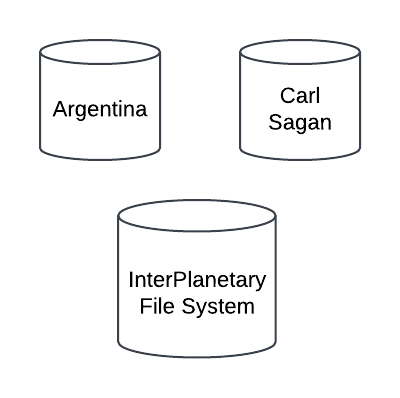
\includegraphics[width=0.4\linewidth]{img/solucion-ipfs/bdd-articulos.png}
    \caption{Representación de cada articulo como su propia base de datos.}
    \label{fig:bdd-articulos}
\end{figure}

De esta manera ya tenemos una representación para los artículos, pero faltaría una forma de saber que artículos existen actualmente. Es por eso que tenemos que agregar una última base de datos, también de eventos, que represente la wiki en si, con los nombres de los artículos existentes. De esta manera un usuario puede saber, al acceder a esta base de datos representando un repositorio de artículos, cuales son los artículos que existen y solo acceder a la base de datos correspondiente a ese articulo, sin necesidad de replicar la totalidad de los artículos existentes, algo que sería inviable.

\begin{figure}[H]
    \centering
    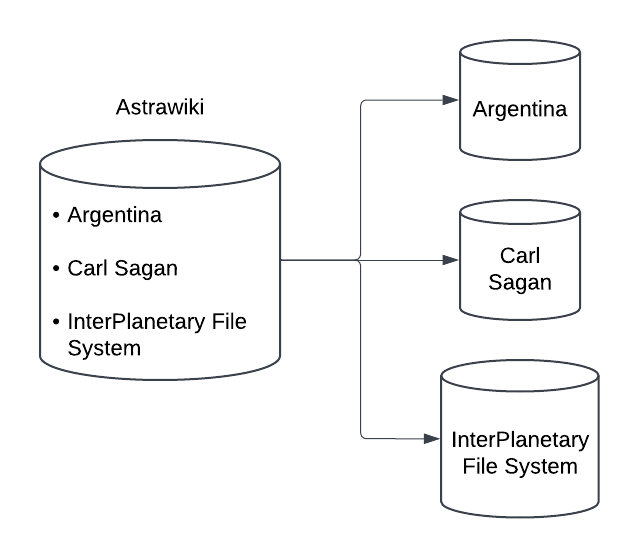
\includegraphics[width=0.6\linewidth]{img/solucion-ipfs/bdd-wiki.png}
    \caption{Representación del repositorio de artículos como base de datos.}
    \label{fig:bdd-wiki}
\end{figure}

Ahora bien, ¿cómo podemos acceder a la base de datos? En OrbitDB las bases de datos tienen una dirección que las identifica, formada en su creación. Esta dirección está conformada por el nombre de la base de datos, su tipo y su \textit{Access Controller}. Este último sirve para indicar quien tiene acceso y permisos sobre la base de datos. Como en nuestro caso estamos permitiendo que todos tengan permiso, el \textit{controller} va a ser siempre el mismo. Esto nos es importante, ya que, como el tipo de la base de datos y su \textit{controller} van a ser siempre los mismos, con solo saber el nombre identificador, al crear la base de datos, vamos a tener siempre la misma dirección, y en consecuencia, vamos a tener siempre la misma base de datos. 

\begin{figure}[H]
\centering
\fbox{\texttt{/orbitdb/zdpuAmrcSRUhkQcnRQ6p4bphs7DJWGBkqczSGFYynX6moTcDL}}
\caption{Ejemplo de la \textit{address} de una base de datos de OrbitDB.}
\end{figure}

Esto nos es de mucha utilidad ya que con saber únicamente el nombre identificador de la wiki, podemos acceder su base de datos, como también a las bases de datos de sus artículos al componer ambos nombres, el de la wiki con el del articulo, y asi acceder a la base de datos del artículo.

\begin{figure}[H]
    \centering
    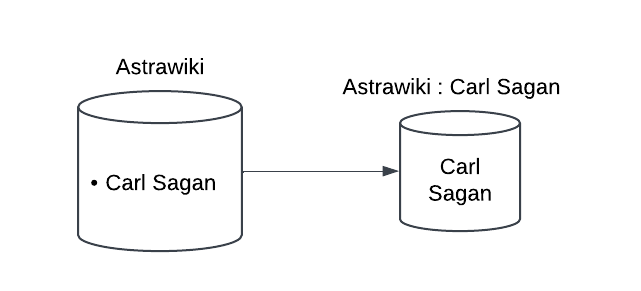
\includegraphics[width=0.6\linewidth]{img/solucion-ipfs/bdd-names.png}
    \caption{Representación de los nombres identificadores de la wiki y sus artículos.}
    \label{fig:bdd-names}
\end{figure}

Es importante notar que en ningún momento vamos a estar abriendo explícitamente una base de datos desde un nodo nuevo, sino que vamos a estar creando la misma base de datos vacia desde cero para luego sincronizarla con el resto de nodos. Esto sucede ya que, si recordamos, OrbitDB es una base de datos \textbf{eventualmente consistente}, lo que significa que OrbitDB te asegura que en algún momento todos los nodos van a converger a la misma información, pero no te da la certeza de cuándo va a suceder. Esto también nos ayuda ya que no podemos nunca estar seguros si somos los primeros al crear una base de datos o si ya existe y aún no fuimos sincronizados, generándose como si fuera un \textit{chicken egg problem}, por lo tanto al tener en cuenta se evita hacer asunciones que pueden generar problemas.

Otro punto importante es que al estar identificando a las bases de datos con su nombre, significa que es muy fácil crear una wiki alternativa que sea totalmente independiente a otras existentes, permitiendo asi total libertad de crear y mantener otras wikis que se quiera, cada una con sus articulos correspondientes y persistida por sus propios colaboradores. Esto nos va a ser de especial utilidad cuando este enfoque no solo lo utlicemos para wikis, el cual explicaremos con detalle más adelante.

\begin{figure}[H]
    \centering
    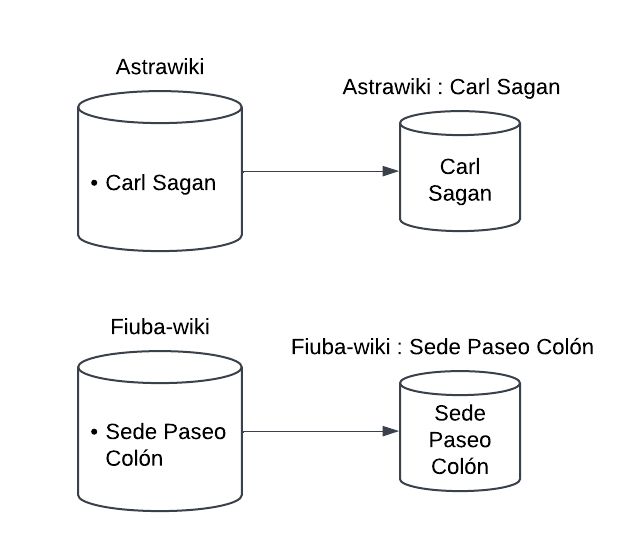
\includegraphics[width=0.6\linewidth]{img/solucion-ipfs/bdd-multiple.png}
    \caption{Representación de múltiples wikis independientes.}
    \label{fig:bdd-multiple}
\end{figure}

\paragraph{Colaboradores}

En orbitdb, al ser una base de datos peer-to-peer, distribuida y sin un servidor central, significa que la base de datos existe en cada peer que la componga, por lo tanto conectarse a una base de datos significa replicar la totalidad de su información de otros peers que nos la provean. De no estar esos peers, significaría que la base de datos no puede ser accedida y su información podría perderse, tal como sucedía cuando explicamos la infraestructura anterior. Es por eso que una gran parte de la arquitectura está pensada al rededor de peers que opten por ser colaboradores, estos peers van a replicar todas las bases de datos que existan actualmente en la base de datos central, pensandolo en el caso del repositorio, van a preservar todos los articulos que existan. De esta manera logramos que mientras haya por lo menos un colaborador en linea, la wiki va a poder ser accedida.

Idealmente no tendría que ser necesario replicar toda la información en cada colaborador, sino que replicarla inteligentemente en suficientes colaboradores proveeria de suficiente persistencia y disponibilidad. Sin embargo y similar a como se explicó anteriormente en el análisis de la infraestructura de despliegue, debido a la falta de \textit{proof of storage} no podemos estar seguros nunca que una base de datos este siendo realmente replicada y por la tanto no podemos permitirnos dividir el almacenamiento utilizado entre distintos colaboradores, ya que seria muy susceptible a la perdida de información si se le asigna la responsabilidad de una base de datos a todos nodos los cuales no están verdaderamente replicandola. Esta decisión conlleva a otros puntos a remarcar de los cuales entraremos en detalle mas adelante.

Estos peers colaboradores son el punto más importante que diferencia esta solución con el resto y que sigue con la filosofía de las aplicaciones comunitarias que estamos analizando, permitiendo que la disponibilidad de la información se este logrando a través de la donación de almacenamiento en vez de dinero.

Es importante remarcar que los colaboradores no tienen ningúna responsabilidad o permisos extra que los usuarios normales no tengan, su única función es ayudar con la disponibilidad de la base de datos, cualquiera que quiera puede colaborar.

Entonces, un usuario que quiera conectarse a la base de datos y obtener su información, por ejemplo querer conectarse a la wiki y ver artículos, debe primero conectarse a alguno de estos colaboradores, de los cuales puede replicar la información a su base de datos propia. Sin embargo esto no es tan trivial como parece, pasemos a ver como se resuelve este problema.

\paragraph{Manejo de conexión}

OrbitDB no se responsabiliza de manejar las conexiones, tampoco le importa, ya que te asegura que eventualmente la base de datos va a estar sincronizada entre peers, aunque se caigan las conexiones o te conectes mas tarde, todo se va a sincronizar sin conflictos eventualmente. Por lo tanto delega esa responsabilidad a \textbf{Helia}\cite{helia} la cual es la implementación de IPFS en los lenguajes javascript/typescript, que a su vez delega la responsabilidad a \textbf{LibP2P}\cite{libp2p} y de la cual tenemos que hacer uso nosotros para manejar las conexiones.

LibP2P es una colección de protocolos y utilidades para facilitar la implementación de una red peer-to-peer. Al crear un nodo de LibP2P se tiene que elegir como conformarlo en base a un conjunto modular de herramientas, dentro de los que se encuentran mecanismos de seguridad, de transporte, descubrimiento de pares, entre otros. Cada una de estas herramientas es importante y hace que el nodo funcione como queramos, más adelante explicaremos la decisión para cada herramienta elegida, sin embargo ahora nos vamos a centrar en dos protocolos de interés necesarios para solucionar el problema de manejo de conexión. Los protocolos de transporte y de descubrimiento de peers.

Los protocolos de transporte son los encargados de la comunicación entre nodos, de manera similar a la capa de transporte presente en toda red convencional. Se basan en tipos de transporte ya existentes, adaptados al uso peer-to-peer. Como lo son TCP, QUIC o WebSockets. Sin embargo no todos los transportes nos son útiles y la decisión de cual protocolo utilizar no es sencilla.

Uno de los requisitos de esta infraestructura era la posibilidad de utilizarla para crear aplicaciones que se puedan utilizar desde un entorno web, como es el caso de un usuario queriendo acceder a la wiki desde un navegador. Lo que sucede es que el entorno web no es muy amigable con las conexiones. Los navegadores están construidos sobre HTTP(S), un protocolo sin estado basado en solicitudes y respuestas. El cliente (navegador) envía una solicitud y luego espera una respuesta. Las conexiones se manejan en la capa de transporte y no mediante HTTP(S). Los navegadores imponen reglas estrictas, como los requisitos de certificados y el bloqueo de políticas de origen cruzado (cross-origin).

Es por esto que por razones de seguridad, no es posible que un navegador establezca una conexión TCP o QUIC sin procesar directamente desde el navegador, ya que todas las conexiones deben cumplir con los requisitos de Contexto Seguro (Secure Context), como por ejemplo que los mensajes se entreguen a través de TLS.

Es por esta razón que la infraestructura debe hacer una diferenciación entre nodos que se ejecuten desde un entorno independiente, como es el caso de \textbf{node.js}\cite{nodejs} y nodos que se ejecuten en un entorno web, únicamente para asignarle los protocolos de transporte correspondientes a su entorno.

Hay 2 conexiones que se tienen que resolver, la conexión entre nodos independientes y la conexión desde un nodo web a un nodo independiente.

Para los nodos independientes la solución es sencilla y el protocolo utilizado es TCP, con el cual pueden comunicarse entre sí y con otros nodos independientes de la red. El problema viene que, como explicamos, TCP no nos sirve para comunicar desde un nodo web a un nodo independiente, por lo tanto hay que explorar alternativas.

Al momento de comenzar con el desarrollo del repositorio de conocimiento, la implementación de LibP2P en javascript ofrecía dos formas para resolver la conexión de web a nodo independiente.

La primera alternativa analizada y más conocida es la de utlizar \textbf{WebSockets}\cite{websocket}. El protocolo WebSocket permite “secuestrar” una conexión HTTP y tras una solicitud para asegurar la conexión, el navegador obtiene acceso directo a la conexión TCP subyacente, permitiendo comunicación bidireccional persistente. Sin embargo esta alternativa no nos de fue de utilidad ya que para lograr esta mejora de conexión es necesario contar con un dominio o certificado por una autoridad certificadora, cosa que muy probablemente los nodos y usuarios utilizando la infraestructura no tengan.

La otra alternativa adicional considerada fue el uso de la técnica conocida como \textbf{Hole Punching}\cite{hole-punching}, una técnica muy interesante que permite que nodos privados —es decir, aquellos ubicados detrás de un firewall o en redes donde no pueden recibir conexiones entrantes, como hogares, redes corporativas o dispositivos móviles— puedan establecer conexiones con otros nodos. Para lograrlo, un nodo público actúa como intermediario, escuchando por ellos, este nodo es denominado como \textbf{Relay}. Esto nos sirve ya que un nodo web actua como un nodo privado ya que, aunque no pueden aceptar conexiones entrantes, sí pueden iniciarlas; así, todo el tráfico pasa a través del nodo intermediario, permitiendo una comunicación efectiva. No obstante, esta opción presenta una limitación relevante: el soporte para esta funcionalidad aún se encuentra en desarrollo en la implementación de libp2p para JavaScript, y no fue posible obtener un funcionamiento estable en el contexto de nuestro proyecto.

Al ver que ambas formas provistas no nos eran de utilidad nos puso en un lugar difícil, dado que de no poder lograr la conexión significaría que esta infraestructura no iba a poder funcionar, sin embargo el desarrollo e investigación continuó aunque no sabíamos si se iba a poder lograr una forma exitosa, lo cual era un riesgo. Sin embargo en al rededor de la mitad del proyecto, el soporte para una nueva alternativa se implementó.

Esta nueva alternativa es la conocida como \textbf{AutoTLS}\cite{autotls} la cual conciste en obtener un certificado y dominio dependiente del ID del nodo usando el protocolo conocido como \textbf{ACME}\cite{acme}, del cual libp2p provee un servicio DNS de bien público que responderá en nombre de cualquier usuario de Internet. De esta manera se puede usar el método de websockets de manera segura gracias al certificado que se obtiene. El funcionamiento de esta alternativa nos permitió continuar con el desarrollo y poder probar la infraestructura que se estaba creando. Sin embargo esta alternativa seguía teniendo algunas desventajas, la primera era que su conexión era muy inestable, al también ser una nueva alternativa experimental sufría de problemas. Pero más importante aún era que iba en contra de la filosofía que intentábamos lograr, que es la de una descentralización, como se requiere de un servidor de terceros para obtener el certificado, se depende de la disponibilidad de este servidor, y de no estar significaría que los nodos no puedan conectarse, por lo tanto aún necesitábamos una mejor alternativa.

Un tiempo después surge el soporte de una nueva alternativa, la cual ya teniamos conocimiento porque existía en otras implementaciones de libp2p en otros lenguajes y estaba en desarrollo para la implementación en javascript. Esta alternativa es la conocida como \textbf{WebRTC}\cite{webrtc} mas especificamente su implementación directa para conectar desde web a nodo independiente llamada \textbf{WebRTC-Direct}.  Curiosamente hasta los mismos desarrolladores de libp2p recomendaban utilizar otras implementaciones en otros lenguajes para resolver la conexión web a nodo independiente hasta que el soporte de esta alternativa o otra muy similar se completen, citando: "Therefore, until WebRTC-Direct or WebTransport support is added to js-libp2p in Node.js, it’s much easier to use go-libp2p."\cite{differences-nodejs-browser} Lo cual no podiamos permitirnos por el requisito de permitir utilizarlo en aplicaciones web y que orbitdb tambien se encuentra en el ecosistema de javascript.

WebRTC es un conjunto de estándares abiertos y APIs web que permiten a las aplicaciones web establecer conectividad directa para conferencias de audio y video, así como para intercambiar datos arbitrarios. LibP2P lo utiliza para lograr una conexión directa y sin necesidad de usar un certificado TLS. De esta manera logramos que ya no sea necesario utilizar AutoTLS y podemos conectarnos corrementamente desde un nodo web a un nodo independiente usando WebRTC-Direct.

De esta manera la topología de conexiones resultante entre nodos independientes y nodos web resulta de la siguiente forma: 

\begin{figure}[H]
    \centering
    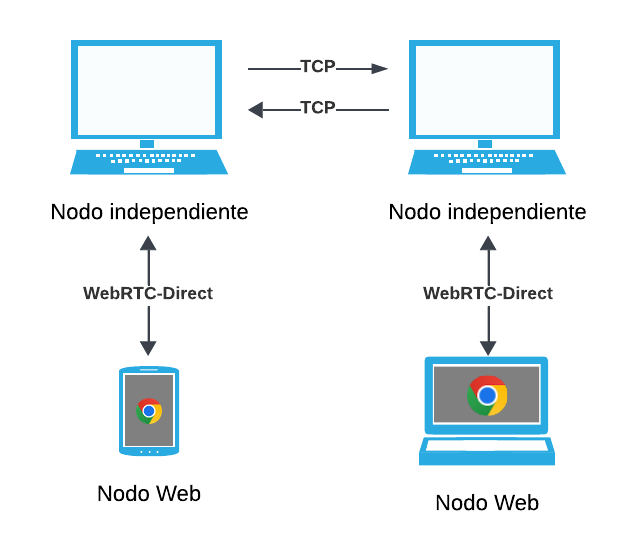
\includegraphics[width=0.5\linewidth]{img/solucion-ipfs/topologia.png}
    \caption{Topología de conexiones entre nodos independientes y nodos web.}
    \label{fig:bdd-articulos}
\end{figure}

Algo a notar es la falta de una conexión entre nodos web, lo cual sería algo muy útil, ya que los mismos usuarios web utilizando la aplicación en un determinado momento, podrian ayudar a proveer de las bases de datos a nuevos usuarios que se conecten y no dejar que solo los nodos independientes puedan hacerlo, lo cual seguría muy bien la filosofía de IPFS, sin embargo esto requeriría que los nodos web puedan escuchar conexiones entrantes y esto es únicamente posible haciendo uso de un \textbf{Relay} como explicamos anteriormente y que actualmente no fue posible obtener un funcionamiento estable en el contexto de nuestro proyecto. Igualmente sería algo muy fácil de implementar una vez que su funcionamiento sea estable y agregaría esta característica que mejoraría la infraestructura.

\paragraph{Descubrimiento de colaboradores}

Hasta ahora explicamos cómo se conectan y que protocolos de transporte utilizan los distintos nodos de nuestra infraestructura, sin embargo aún falta algo muy importante del manejo de conexión, el cual es cómo un nodo sabe a que nodo debe conectarse para poder sincronizarse y obtener la base de datos, en esencia, cómo descubre a los colaboradores a los que debe conectarse.

Una primera idea puede venir de dejar públicos algunas direcciones de nodos que sepamos que son colaboradores, por ejemplo nodos creados por nosotros, lo cual traería bastantes problemas. El problema más importante con este enfoque es que se estaría rompiendo completamente la descentralización de la infraestructura, ya que su disponibilidad pasaría a depender únicamente de la disponibilidad de estos \textit{bootstrap nodes}, por lo tanto hay que lograr encontrar otro enfoque que respete con la descentralización que estamos buscando lograr.

Una alternativa más alineada con los principios de descentralización puede encontrarse al analizar cómo el sistema IPFS resuelve el problema de descubrimiento de contenido en su red. Como se explicó previamente, IPFS se basa en el concepto de content addressing \cite{content-addressing}, es decir, los datos son accedidos mediante su contenido (identificado de forma única por un Content Identifier o CID) en lugar de su ubicación específica. La localización del contenido se realiza a través de una Distributed Hash Table (DHT), donde los nodos que poseen determinado contenido se anuncian como proveedores de su correspondiente CID.

La DHT de IPFS funciona como una base de datos distribuida que permite localizar contenido de forma descentralizada. En lugar de un servidor central, cada nodo almacena una fracción del índice global que vincula CIDs con los nodos que los proveen. Así, cuando un nodo desea acceder a un determinado contenido, consulta la DHT para identificar los proveedores del CID correspondiente.\cite{dht}

Este mecanismo puede aprovecharse directamente para resolver el problema del descubrimiento de nodos colaboradores. Si consideramos que el CID representa la base de datos, construida a partir de su nombre identificador, y los colaboradores son los proveedores de dicho CID, entonces basta con realizar una búsqueda en la DHT para obtener una lista de nodos actualmente activos que están ofreciendo ese contenido. De este modo, se logra un enfoque completamente descentralizado en el que los nodos colaboradores pueden anunciar su disponibilidad, y los nuevos nodos pueden descubrirlos e iniciar la sincronización sin depender de un punto central ni de direcciones de nodos preconfiguradas.

\paragraph{AstraDB}

Gracias al análisis anterior, se logró construir una implementación para el repositorio de conocimiento que mantuviera un estado y permitiera su modificación de una manera distribuida y descentralizada. Esta implementación era parte de la solución del repositorio de conocimiento y formaba una gran parte de su arquitectura, sin embargo al empezar con el desarrollo del mensajero en tiempo real, nos dimos cuenta que se podía crear una abstracción para que ambos casos de uso la utilicen, ya que todos los principios iban a ser los mismos, tanto la representación de los datos, como el manejo de conexión y uso de colaboradores. Es así como surge AstraDB.

AstraDB es la abstracción resultante de pensar la representación de los datos como pares clave valor. Donde en vez de tener un repositorio de artículos general, en donde se encuentre el nombre de todos los artículos y cada artículo como su propia base de datos, tengamos un base de datos general en donde se encuentren todas las claves que existen actualmente y una base de datos por cada clave con el contenido de dicha clave. Si bien sería similar a como se compone una base de datos clave valor, esta tiene una importante diferencia, la cual es que los valores de clave se agregan a los anteriores en vez de remplazar el valor actual, esto sucede ya que se sigue respetando el uso de \textit{append only} que nos permitía no tener que generar permisos para evitar el borrado de información y lograr una descentralización.

Su interfaz consiste de dos métodos principales, los cuales permiten el agregado de una nueva clave y obtención de los valores asociados a esa clave. Permitiendo de esta manera que la creación de nuevos casos de uso orientados al uso colaborativo y siguiendo los principios mostrados sea mucho mas fácil y rápido, 
logrando que el foco del desarrollo este en los requisitos del mismo y no en el funcionamiento del ecosistema.

Lo que se tiene que hacer es adaptar el caso de uso al paradigma de clave valor. En el caso del repositorio de conocimiento, como se explicó anteriormente, cada clave representa un artículo, y el contenido del mismo es cada actualización que se le realizó al mismo. Para el caso del mensajero en tiempo real, cada clave representa un determinado chat, con el nombre del chat como la clave, y su contenido representa cada mensaje enviado secuencialmente. Mientras el caso de uso se pueda representar con dicho paradigma, se puede utilizar astradb para su persistencia de forma colaborativa.

\begin{figure}[H]
    \centering
    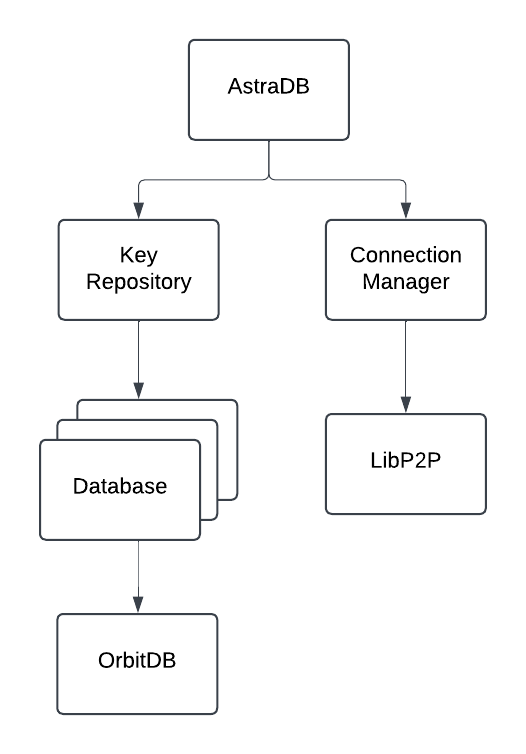
\includegraphics[width=0.5\linewidth]{img/solucion-ipfs/astradb-arquitectura.png}
    \caption{Arquitectura de AstraDB.}
    \label{fig:astradb-arquitectura}
\end{figure}

Su arquitectura, al igual que la descrita anteriormente, consiste de 2 principales ramas, una encargada del manejo de datos y otra del manejo de conexión. Al iniciar el nodo, este inicializa tanto el \textit{Key Repository}, como el \textit{Connection Manager} los cuales funcionan independientemente uno del otro y en paralelo para lograr en conjunto, el funcionamiento de AstraDB.

\paragraph{Key Repository}

Dentro del \textit{Key Repository} se encuentra todo el manejo de datos de la infraestructura. Se encarga de mantener un registro de todas las claves existentes y de realizar las modificaciones requeridas.

Al inicializarse crea la base de datos central con el nombre identificador recibido por parámetro e intenta sincronizarla con los colaboradores conectados. Si no logra sincronizarse con ningún colaborador se asume que es una nueva base de datos y continua con su funcionamiento.

Si al crear el nodo de AstraDB se optó por ser colaborador, al recibir una actualización de la base de datos central sobre una nueva \textit{key} creada, la base de datos representando el contenido de la \textit{key} será abierta y guardada. De esta manera se logra la persistencia de la \textit{key} y  perimite que usuarios puedan acceder a ella al sincronizarse con este nodo.

Las base de datos utilizadas por el \textit{Key Repository}, tanto la central como las de cada \textit{key} individual, están representadas por una abstracción llamada \textit{Database}. En esta abstracción se maneja toda interacción con la base de datos de OrbitDB.

Al incializarse se debe optar por si se desea sincronizar la base de datos o si no es necesario. Si se sincroniza entonces se va a esperar que la base de datos se sincronice con algun colaborador conectado, lo que significa obtener todas las actualizaciones que contiene la instancia de base de datos contenida en el colaborador. Una vez sincronizada esta ya permite su funcionamiento, el agregado de nuevo contenido a la base de datos u obtención de todo el contenido del mismo.

OrbitDB permite escuchar por eventos emitidos por la instacia de la base de datos, en nuestro caso es de suma importancia cuando se recibe una nueva actualización, que sucede al sincronizarse con otro usuario y se recibe al menos un nueva entrada a la base de datos, sin embargo una actualización no es siempre el ultimo valor agregado a una base de datos. Por la naturaleza de las bases de datos de OrbitDB y su eventual consistencia, significa que al sincronizarse ambas bases de datos van a tener el mismo contenido y en el mismo orden. Aunque estemos usando una base de datos de tipo eventos y solo se pueda agregar al final, no significa que si dos de esas instancias de bases de datos tienen su contenido propio y aun no fueron sincronizados entre si, al sincronizarse puede que nuevo contenido quede por debajo de contenido nuevo. Es por esto que desde la abstracción se debe tomar recaudos para que no quede contenido nuevo sin notificar, independientemente de su vejez.

Esto es de suma importancia para cuando se utiliza para el mensajero en tiempo real, ya que AstraDB permite escuchar por actualizaciones en tiempo real para una determinada clave, recibiendo de esta forma todas las actualizaciones de un determinado chat.

Para lograr esto la abstracción \textit{Database} mantiene un registro de todas las claves vistas hasta un determinado momento, en OrbitDB cada entrada a una base de datos tiene un hash identificador y es eso lo que nos guardarnos. Al recibir un evento de \textit{Update} desde la base de datos de OrbitDB, debemos iterar todas las entradas que contiene dicha base de datos para encontrar si hay entradas nuevas, no antes vistas. Se debe iterar en su totalidad ya que nada asegura que no haya entradas nuevas en distintas posiciones de la base de datos, como vemos que puede suceder en el siguiente ejemplo:

\begin{figure}[H]
    \centering
    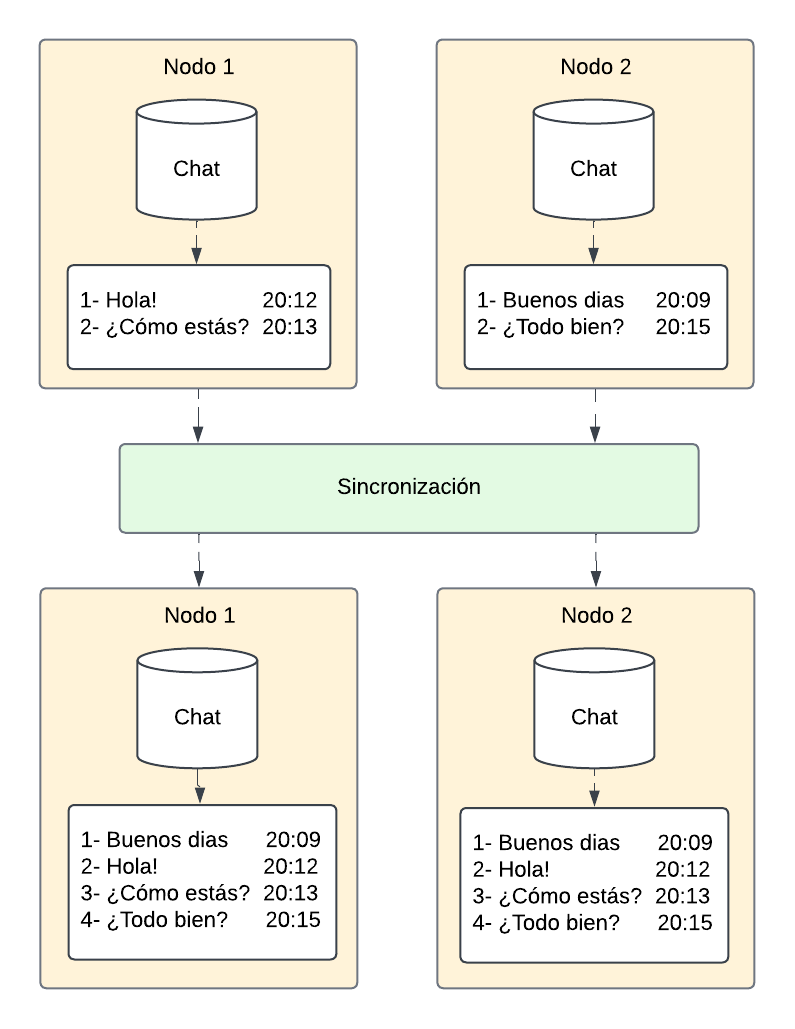
\includegraphics[width=0.7\linewidth]{img/solucion-ipfs/ejemplo-sincronizacion.png}
    \caption{Ejemplo de sincronización de nodos.}
    \label{fig:ejemplo-sincronizacion}
\end{figure}

En el ejemplo contamos con dos nodos independientes que forman parte de la misma base de datos con nombre 'Chat'. Cada nodo tiene su propia representación de la base de datos hasta un determinado momento. A continuacion se puede observar que ocurre una sincronizacion entre ambos nodos, esto hace que ambos nodos pasen a tener la misma representacion de informacion de la base de datos fusionando lo que tenian previamente, de esto se encarga OrbitDB. Lo importante a notar aca es que desde el punto de vista del nodo 1, las entradas nuevas de la base de datos no estan al final de la misma unicamente, sino que aparece una nueva entrada previa a sus entradas que tenia. Y como se mencionó anteriormente, OrbitDB solo anuncia el evento \textit{Update} al sincronizarse con otro nodo y con únicamente la última entrada actualizada, en este caso avisaría del último mensaje con contenido '¿Todo bien?'. Es por esto mismo que desde la abstracción \textit{Database} es necesario recorrer todas las entradas actuales para encontrar aquellas nuevas en la instancia de base datos propia y avisar por un evento individualmente por cada una. 

\paragraph{Connection Manager}

Dentro del \textit{Connection Manager} se encuentra todo el manejo de conexiones de la infraestructura. Se encarga de encontrar y conectarse a otros colaboradores que provean la base de datos utilizada, como también agregarse como proveedor si se trata de un nodo colaborativo.

Al inicializarse lo primero que hace es construir el \textbf{CID} identificador de la base de datos central, para esto utiliza \textbf{Helia}\cite{helia}, la implementación de IPFS para javascript, para codificar el nombre identificador recibido por parámetro. Como se explicó anteriormente, este CID va a ser siempre el mismo para todas las instancias de AstraDB que utilicen el mismo nombre identificador.

Luego inicializa tres servicios que van a estar funcionando en paralelo durante la ejecución de AstraDB. Esos servicios son: \textit{SearchForProviders}, \textit{ProvideDB} y \textit{ReconnectToProviders}.

En \textit{SearchForProviders} se va a realizar una busqueda continua de nuevos proveedores de la base de datos que se está utilizando, para conectarse a ellos y poder sincronizarse. Para esto va a realizar una consulta a la \textbf{DHT} utlizando \textbf{LibP2P}\cite{libp2p}, buscando los proveedores del CID construido anteriormente. Al encontrar un nuevo proveedor, se va a intentar conectarse a este.

En \textit{ProvideDB}, solo en caso de optar por ser colaborador, se va a notificar utilizando la \textbf{DHT} que el nodo es un proveedor de la base de datos utilizada. De esta manera otros nodos pueden encontrar al nodo utilizado en su busqueda de proveedores.

Por último, en \textit{ReconnectToProviders} se va a estar iterando una lista de proveedores previamente conectados para intentar reconectarse a ellos, por si ocurrió una falla en la conexión.

\paragraph{Resultado}

Como resultado del análisis y creación de esta infraestructura, se logró proveer de una herramienta para facilitar la creación de nuevas aplicaciones con enfoque comunitario, distribuido y descentralizado utilizando el ecosistema de IPFS. De la cual nuestros casos de uso Astrawiki y Astrachat la utilizan para su funcionamiento.

\paragraph{Limitaciones}

Sin embargo este enfoque presenta algunas limitaciones o aspectos a mejorar que son importantes destacar.

Para la solución implementada, la seguridad no fue una prioridad. En consecuencia se presentan algunos problemas que están relacionados con esto. La solución da total libertad a la creación y agregado de información a las bases de datos sin ninguna limitación, junto a que los colaboradores deben almacenar la totalidad de la base de datos, por lo que se explicó anteriormente de la falta de \textit{Proof of storage}, lo cual de por si es un limitación. En consecuencia es muy fácil realizar un ataque de spam, usando el espacio almacenado de los colaboradores, al crear nuevas \textit{Keys} o agregar contenido sin importancia a cada una de ellas. Esto podría mitigarse si se utilizara un consenso a la hora de aceptar un cambio o no a la base de datos, dado que si el cambio no se acepta, entonces no se distribuye y no se efectúa, sin embargo, como se explicó, esto requiere un foco de seguridad y para mostrar su uso en el ecosistema no fue el punto principal.

Relacionado con lo anterior, permitir la modificación libre de toda la información puede que no sea lo deseado para otro tipo de aplicaciones. Si se quisiera crear un blog personal o de microblogging, se desearia que solo  pueda moficar la información el dueño del blog y que los colaboradores solo ayuden con la persistencia del mismo. Esto puede ser una posible mejora y es posible si se puediera optar que las bases de datos de las keys tengan el permiso de moficiacion unicamente al usuario que las creó, como tambien referenciar a la \textit{Address} de la base de datos creada, ya que en este caso si depede de su creador, por lo que se explicó en anterioridad en la representación de los datos.

Tambien tiene una limitacion con que no se pueden crear cosas privadas, dado que el almacenamiento esta en la red de ipfs y cualquiera puede acceder a el y la falta de encirptacion, hace que para casos de uso donde se requiera privacidad de informacion no es lo ideal.

\subsubsection{Colaboración}

Se creó una herramienta para facilitar la colaboración a nuestra wiki. El nodo es capaz de fijar los contenidos de Astraweb, nuestro front-end, y también mantener todas las bases de datos utilizadas por Astrawiki y Astrachat en la capa de aplicación. Para lograr esto, se diseñó un sistema con cuatro contenedores, cada uno asignado a uno de los tres casos de uso.

Para el pinning del sitio web en si, se utilizó el contenedor de IPFS Cluster con la instrucción de colaborar con el clúster dado por parámetro. Este parámetro es la dirección IPFS del archivo \texttt{service.json} que identifica a un clúster. Además, IPFS Cluster requiere de un contenedor de Kubo para manejar el manejo de archivos en la red de IPFS.

Para Astrawiki, se hizo uso del contenedor ofrecido por Astrawiki CLI, front-end que se verá más adelante. Con este contenedor, se puede actuar como colaborador fácilmente sin necesidad de interactuar con él.

Por último, Astrachat se levanta con un simple proyecto de Node que crea un nodo colaborativo y lo ejecuta en segundo plano.

\begin{figure}[H]
    \centering
    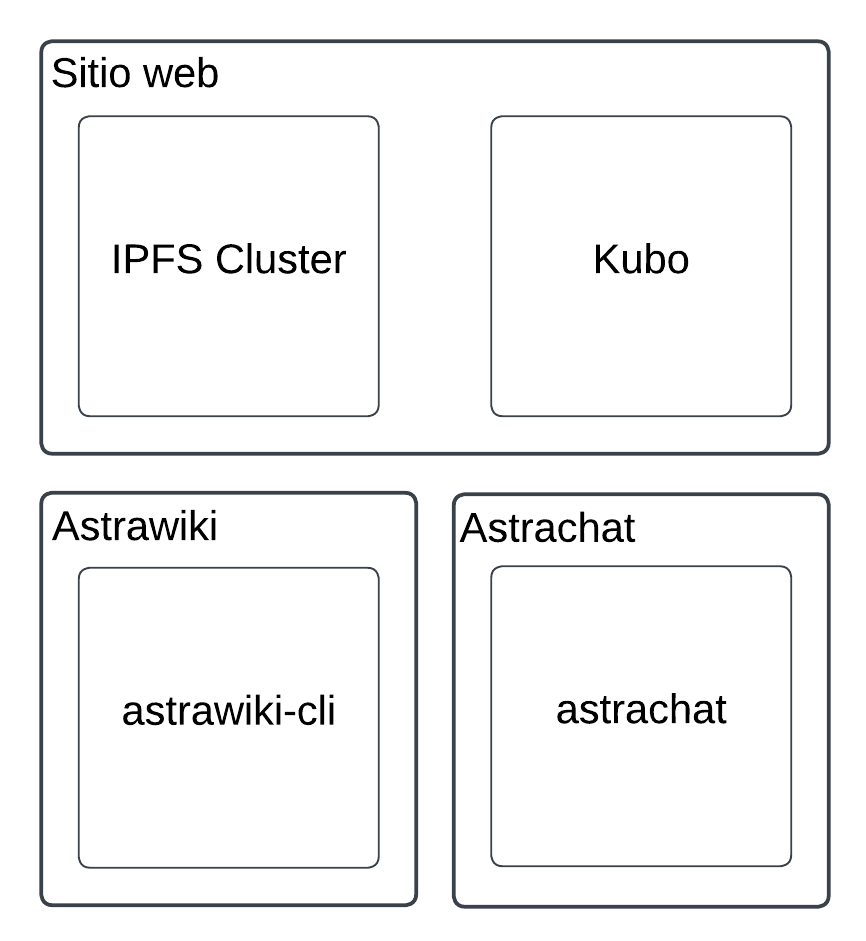
\includegraphics[width=0.5\linewidth]{img/solucion-ipfs/collaborator-arch.png}
    \caption{Arquitectura general del nodo colaborador}
    \label{fig:collaborator-architecture}
\end{figure}

Cada uno de estos casos se puede seleccionar o deseleccionar desde un archivo de configuración \texttt{.env}, para que el usuario pueda elegir en que parte del proyecto contribuir. El resultado es una herramienta que, si bien fue diseñada para Astraweb, puede utilizarse para cualquier tipo de front-end que utilice Astrawiki y/o Astrachat.